\chapter{IEC 61850 -standardi}
\label{ch:iec61850-theory}
% Aihepiirijärjestys tutusta uuteen.
% Tuttuja asioita: sähköasema, julkaisija-tilaaja-paradigma, viestejä voidaan tilata.
% Luvussa käsiteltävät asiat.
IEC 61850 -standardi määrittää säännöt, kuinka sähköaseman laitteet kommunikoivat keskenään verkon yli. Standardi koskee myös aseman kanssa kommunikoivia ohjelmistoja. Standardi on laaja monesta dokumentista koostuva kokonaisuus. Tämän takia tässä luvussa standardista käsitellään vain diplomityön kannalta tärkeitä asioita. Käsittely aloitetaan yleiskuvalla ja edetään tärkeään asiaan. Saatuja tietoja tullaan käyttämään myöhemmin pohjana järjestelmän arkkitehtuurin ja ohjelmiston suunnittelussa.


\section{Yleiskuva}
% Sähköaseman IED-laitteet toteuttavat aseman toiminnallisuutta.
Sähköaseman tehtäviin kuuluu mm. jännitteen muuntaminen, verkon jakaminen ja sen toiminnan tarkkailu. Virhetilanteissa aseman laitteisto toimii estääkseen suuremman vahingon. Näitä laitteita sähköasemalla ohjaa ja tarkkailee sen automaatiolaitteet, joita kutsutaan \emph{älykkäiksi elektroniikkalaitteiksi} (\emph{Intelligent Electronic Device}, \emph{IED}). IED:t on kytketty sähköverkon laitteisiin joita ne ohjaavat. Näitä laitteita on mm. muuntajat ja katkaisijat. IED:t myös kytketään verkkoon, jotta ne voivat kommunikoida keskenään ja asemalta ulospäin. Asemalta ulospäin kommunikointi mahdollistaa sen etäohjauksen ja tarkkailun ohjelmiston avulla.

% Standardi IED-laitteiden kommunikoinnin määrittämiseen.
% Standardia voi toimia monella eri tekniikalla, mutta käytetään MMS-protokollan avulla.
IEC 61850 -standardi määrittää kuinka IED-laitteet ja etäohjelmistot kommunikoivat keskenään. Standardin tarkoitus on asettaa yhteiset säännöt, jotta eri valmistajien laitteet ja ohjelmistot olisivat yhteensopivia keskenään. Standardi on määritetty tekniikasta riippumattomaan muotoon, joka erikseen mallinnetaan halutulle tekniikalle. Mallinnuksia on olemassa eri tekniikoille, mutta tässä työssä kommunikointi tapahtuu pelkästään MMS-protokollan (Manufacturing Message Specification) päällä. MMS-protokolla on TCP/IP-protokollaperheen päällä toimiva kommunikointiprotokolla.

% Viestien tilauksen pääpiirteinen toiminta.
Standardi määrittää säännöt kuinka asiakasohjelmat voivat tilata viestejä IED-laitteelta verkon yli. Viestien tilaus noudattaa julkaisija-tilaaja-paradigmaa, jossa IED-laite on julkaisija ja asiakasohjelmat tilaajia. Julkaisija-tilaaja-paradigma käsiteltiin aikaisemmin kappaleessa \ref{ch:julkaisija-tilaaja-paradigma}. Viestien sisältö on IED-laitteessa olevaa tietoa, kuten mittausdataa tai siihen kytketyn laitteen tilatietoa. Viestit tilataan IED-laitteelta olevalta muuttujalta, joka konfiguroidaan ennen tilausta. 
Standardi asettaa rajoituksia tilaajien määriin, jotka täytyy ottaa huomioon ohjelmiston suunnittelussa. Jotta näitä rajoituksia ja tilauksen toimintaa voidaan ymmärtää, täytyy ensin tarkastella, kuinka standardi määrittää muuttujia IED-laitteeseen.


\section{Sähköaseman laiteiden mallinnus}
% Muuttujilla IED-laite mallintaa aseman laitetta.
Muuttujilla IED-laite mallintaa siihen kytkettyä sähköaseman laitetta kuten katkaisijaa tai muuntajaa. Muuttujat esittävät mm. linjasta mitattua jännitteen arvoa tai katkaisijan tilaa, joka voi olla auki tai kiinni. IED-laitteessa olevien muuttujien määrä vaihtelee sen mukaan mitä laitetta sen on tarkoitus ohjata.

% Muuttujat muodostuvat valmiiksi määritetyistä luokista.
Mitä muuttujia IED-laite sisältää määrittyy standardin mukaan. Standardi esittää luokkamäärityksiä kaikille sähköaseman laitteille mm. katkaisijoille ja muuntajille. Luokka määrittää mitä muuttujia sen instanssi tulee sisältämään ja jotka kuvaavat kyseistä laitetta. Luokasta muodostetaan instanssi IED-laitteelle sen mukaan, mitä laitetta se ohjaa. Esimerkiksi jos IED-laite ohjaa linjan katkaisijaa, määritetään IED-laitteeseen standardin määrittämä katkaisijaluokan instanssi. Tällöin IED-laite sisältää muuttujia katkaisimen tilasta ja sen ohjauksesta.

% Luokkat muodostavat hierarkian ja koostuvat toisistaan.
Standardin luokkamääritykset sisältävät aliluokkia ja jotka taas sisältävät muuttujia tai muita aliluokkia. Standardissa luokkamääritykset toimivat samalla periaatteella kuin oliohjelmoinnin luokat. Luokat sisältävät samaan asiaan liittyviä muuttujia ja toiminnallisuutta. Näistä luokista ja muuttujista standardissa muodostuu oliopohjainen hierarkkinen rakenne. Esimerkiksi muuntajaa mallintava luokka sisältää aliluokkia mittaustiedon esittämisestä. Samaa aliluokkaa käytetään jonkin muun mittaustietoa sisältävän laitteen mallintamiseen. Voidaan sanoa, että standardin mukainen laitteen luokka koostuu muista aliluokista. Kun laitteen mallintavasta luokasta tehdään instanssi IED-laitteelle, samalla myös tehdään instanssi kaikista sen aliluokista. IED-laite siis sisältää myös kaikki aliluokkien muuttujat.

\section{Muuttujien yksilöinti IED-laitteessa}
% Viittaus muuttujiin hierarkiassa.
IED-laite siis sisältää muuttujia hierarkiassa sen mukaan mitä laitetta se ohjaa. Näitä muuttujia voidaan lukea ja kirjoittaa standardin määrittämillä palvelukutsuilla. Jotta voidaan yksilöidä mitä muuttujia halutaan kutsulla lukea tai kirjoittaa, muuttujia täytyy pystyä yksilöimään hierarkiassa. Tätä varten standardi määrittää viittaustekniikan, jota käytetään kutsun yhteydessä yksilöimään mitä muuttujia se koskee. Tämä viittausformaatti on määritetty kuvassa \ref{fig:iec61850-data-reference}. Viittaus muodostuu hierarkiassa olevien luokkien instanssien ja muuttujien nimistä. Nimiä yhdistetään peräkkäin, jolloin viittausta voidaan seurata lukemalla minkä luokan instanssin mitä muuttujaa halutaan lukea tai kirjoittaa. Ensimmäisen ja toisen nimen väliin tulee kauttaviiva (/) ja loput yhdistetään pisteellä (.).

\begin{figure}[ht!]
	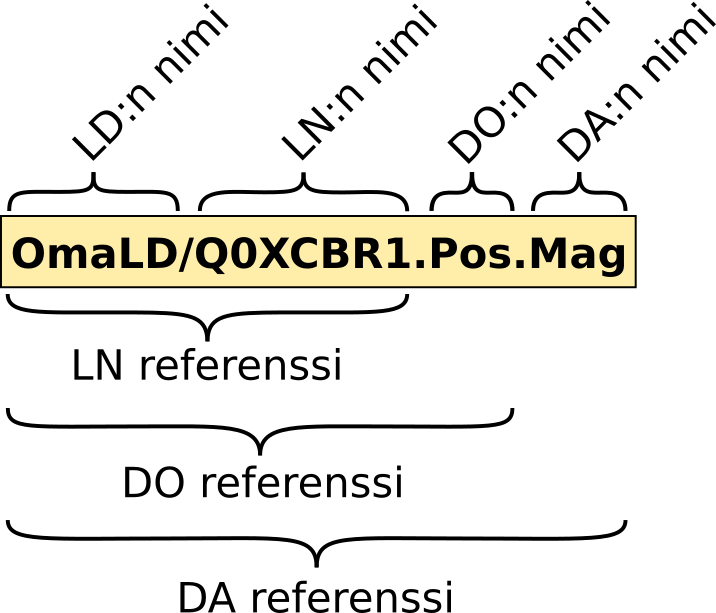
\includegraphics[width=0.5\textwidth]{pictures/iec61850-data-reference.png}
	\caption{IEC 61850 -standardin määrittämä viitteen rakenne (pohjautuu kuvaan \mbox{\cite[s.~93]{IEC61850-7-1}}).}
	\label{fig:iec61850-data-reference}
\end{figure}

% Viittauksen käsitteet lyhyesti.
Viite muodostuu käsitteistä:
\begin{itemize}
	\item \emph{looginen laite} (\emph{Logical Device}, \emph{LD}),
	\item \emph{looginen noodi} (\emph{Logical Node}, \emph{LN}),
	\item \emph{dataobjekti} (\emph{Data Object}, \emph{DO}) ja
	\item \emph{data-attribuutti} (\emph{Data Attribute}, \emph{DA}).
\end{itemize}
viitteessä vasemmalta oikealle järjestyksessä. Käsitteet ovat standardissa tapa esittää minkä tason luokka tai muuttuja hierarkiassa on kyseessä. Tämä tieto on diplomityön ulkopuolella ja lukija voi ne tarkistaa tarvittaessa standardista. Kuitenkin lyhyesti \emph{looginen laite} esittää jotakin aseman fyysistä kokonaisuutta, jota IED-laite ohjaa. \emph{Looginen noodi} on luokka laitteesta kuten muuntajasta tai katkaisijasta. \emph{Dataobjekti} on luokka joka sisältää muuttujia samaan asiaan liittyen, esimerkiksi mittaukseen. \emph{Data-attribuutti} on muuttuja, joka sisältää arvon mitatusta jännitteestä tai katkaisijan tilasta.


\section{Viestien tilaus}
% Viestin tilauksen luokan toiminta.
Standardi määrittää luokkia eri asioiden mallintamiseen, joista tehdään instansseja IED-laitteelle tarpeen mukaan. Samaa periaatetta noudattaen standardi määrittää myös luokan, joka vastaa viestien tilauksesta. Luokasta on tehty instanssi muuttujien hierarkiaan ja sillä on nimi. Luokan instanssi sisältää sisältää muuttujia tilauksen konfigurointiin, aloittamiseen ja lopettamiseen. Näitä muuttujia tilajaa voi kirjoittaa ja lukea palvelukutsuilla jotka viittaavaat viestiluokan instanssiin. Esimerkki viitteestä viestiluokan arvojen kirjoittamiseen voi olla \emph{OmaLD/LLN0.BR.OmatViestit}.

% Viestiluokkien datajoukot.
Viestiluokka vastaa tilaajan tilauksen konfiguroinnista ja viestien lähettämisestä. Sisältö viestiin tulee standardin määrittämistä \emph{datajoukoista} (\emph{data set}). IED-laitteelle on mahdollista määrittää standardin mukaisia datajoukkoja. Datajoukko on kokoelma IED-laitteella olevista muuttujista, jotka on kerätty yhteen niiden tärkeyden takia, esimerkiksi kaikki mittauspisteet voivat kuulua yhteen datajoukkoon. Viestiluokka konfiguroidaan tarkkailemaan yhtä tällaista datajoukkoa, josta tilaaja on kiinnostunut. Datajoukossa tapahtuneen muutoksen myötä viestiluokka luo viestin, johon se sisällyttää muuttuneet arvot ja lähettää sen tilaajalle. Esimerkki tästä on jännitteen mitatun arvon muuttuminen uuteen, jonka tarkkaileva viestiluokka huomaa. Seurauksena viestiluokka luo uuden viestin, sisällyttää muuttuneet arvot viestiin ja lähettää sen tilaajalle. Sama toistuu minkä tahansa datajoukon muuttujan muuttuessa.

% Viestiluokan rajoitteet.
Standardi asettaa rajoitteita viestiluokan instanssiin. Yksi viestiluokan instanssi voi palvella vain yhtä tilaaja kerrallaan. Instanssi niin sanotusti varataan tilauksen aloitushetkellä, jolloin muiden tilaajien kirjoitus luokkaan estetään, niin kauan kunnes nykyinen tilaaja lopettaa tilauksen tai yhteys katkeaa. Monen tilaajan halutessa saman datajoukon tiedot muutoksista, täytyy IED-laitteeseen määrittää viestiluokan instansseja tarpeiden mukaan ja konfiguroida ne tarkkailemaan samaa datajoukkoa. Kuvassa \ref{fig:rcb-to-one-dataset} on esitetty tilanne, jossa kolme tilaaja tilaavat saman datajoukon käyttäen kolmea eri viestiluokan instanssia. Kuvassa neljäs tilaaja ei voi kirjoittaa jo varattua viestiluokkaa, jotan sen ei ole mahdollista tilata datajoukosta tulevia viestejä.

\begin{figure}[ht!]
	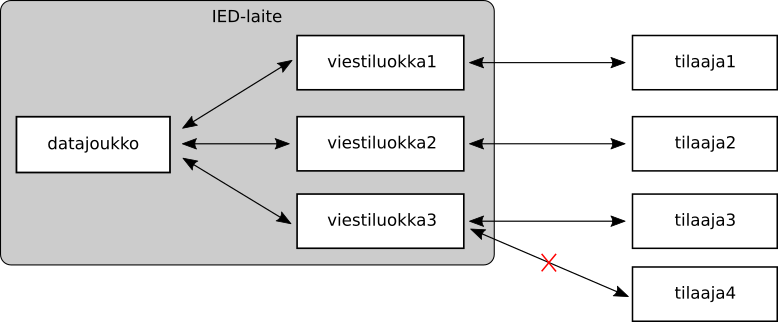
\includegraphics[width=1\textwidth]{pictures/rcbs-to-one-dataset.png}
	\caption{Kolme viestiluokkaa IED-laitteessa palvelee kolmea tilaajaa samasta datajoukosta.}
	\label{fig:rcb-to-one-dataset}
\end{figure}

% Huomioon otettavat rajoitukset suunnitelussa. (yhteenvetoon?)


\section{Viestien sisältö}
% Viestin sisältö.


\section{Yhteenveto}
% Yhteenveto rajoitteista ja toiminnasta.



Sähköasemilla nykypäivänä käytössä olevilla IED-laitteilla toteutetaan aseman toiminnallisuuden funktioita. Aseman toiminnallisuuteen liittyy sen kontrollointi ja suojaus. Aseman komponenttien suojauksen lisäksi, siihen kuuluu myös asemalta lähtevät sähkölinjat. Hyvä esimerkki sähköaseman suojauksesta on korkeajännitelinjan katkaisija, joka katkaisee virran linjasta vikatilanteissa. Tällainen vikatilanne on esimerkiksi linjan poikki meneminen kaatuneen puun tai pylvään takia. Fyysistä katkaisijaa ohjaa aseman automatiikka, joka toteutetaan IED-laitteilla. IED-laite voi olla kytketty fyysisesti ohjattavaan laitteeseen \mbox{\cite[s.~63--64]{IEC61850-7-1}}. Koko sähköaseman toiminnallisuus koostuu monesta eri funktiosta, jotka on jaettu monelle IED-laitteelle. Jotta systeemi pystyy toimimaan, täytyy IED-laitteiden kommunikoida keskenään ja vaihtaa informaatiota toistensa kanssa. IED-laitteiden täytyy myös kommunikoida asemalta ulospäin erilliselle ohjausasemalle monitorointia ja etäohjausta varten \mbox{\cite[s.~1]{Brunner2008}}. On selvää, että monimutkaisen systeemin ja monen valmistajan kesken tarvitaan yhteiset säännöt kommunikointia varten.

Maailmanlaajuisesti asetettu IEC 61850 -standardi määrittää sähköaseman sisäisen kommunikoinnin säännöt IED-laitteiden välillä. Standardi määrittää myös säännöt asemalta lähtevään liikenteeseen, kuten toiselle sähköasemalle ja ohjausasemalle \mbox{\cite[s.~10]{IEC61850-7-1}}. Ilman yhteistä standardia, jokainen valmistaja olisi vapaa toteuttamaan omat säännöt ja protokollat kommunikointiin. Seurauksena olisi, että laitteet eivät olisi keskenään yhteensopivia eri valmistajien kesken. Standardin tarkoitus on poistaa yhteensopivuusongelmat ja määrittää yhteiset säännöt kommunikoinnin toteuttamiseen \mbox{\cite[s.~1]{Kaneda2008}}.

Tärkeä osa standardia on sähköaseman systeemin funktioiden abstrahointi mallien kautta. Standardi määrittää tarkasti kuinka abstraktit mallit määritellään aseman oikeista laiteista ja niiden ominaisuuksista. Tarkoituksena on tehdä mallit tekniikasta ja toteutuksesta riippumattomaksi. Tämän jälkeen määritellään kuinka mallit toteutetaan erikseen toimivaksi jollekin tekniikalle. Abstrahoituja malleja käytetään myös määrittämään sähköaseman IED-laitteiden ja aseman muiden osien konfigurointi. Tekniikasta riippumattomien mallien ansiosta standardi on pohjana tulevaisuuden laajennoksille ja tekniikoille. Uusien tekniikoiden ilmaantuessa, voidaan standardiin lisätä  osa, joka  toteuttaa abstraktimallit kyseiselle tekniikalle \mbox{\cite[s.~2]{Brunner2008}}. Tässä työssä standardin malleja ja palveluita käytettiin \emph{MMS}-protokollan (engl. \emph{Manufacturing Message Specification}) toteutuksella. MMS-protokolla on maailmanlaajuinen \emph{ISO 9506} -standardi, joka on määritetty toimivaksi TCP/IP:n pinon päällä \mbox{\cite{MMS-protocol-stack-and-API}}. Jokainen verkkoon kytketty IED-laite tarvitsee IP-osoitteen kommunikointiin.


\section{Standardin eri osat ja niiden merkitykset}	
IEC 61850 -standardi on laaja kokonaisuus. Tämän takia se on pilkottu erillisiin dokumentteihin, joista jokainen käsittelee omaa asiaansa. Historian saatossa standardiin on lisätty uusia dokumentteja laajentamaan standardia \mbox{\cite{IEC61850series, New-documents-by-IEC-TC-57}} \mbox{\cite[s.~13]{IEC61850-1}}. Tämän työn kirjoitushetkellä standardiin kuului lisäksi paljon muitakin dokumentteja, esimerkiksi uusiin toteutuksiin muille tekniikoille ja vesivoimalaitoksien mallintamiseen liittyviä dokumentteja. Laajuudesta huolimatta standardin voi esittää 10:llä eri pääkohdalla ja näiden alakohdilla. Taulukossa \ref{tab:iec61850-dokumentin-osat} on esitetty standardin pääkohdan dokumentit ja niiden alkuperäiset englanninkieliset otsikot \mbox{\cite{IEC61850series}}. Tässä työssä tullaan viittaamaan standardin eri osiin, jotta lukija voi tarvittaessa etsiä tietoa asiasta tarkemmin.

\begin{table}[ht!]
	\caption{IEC 61850 -standardin pääkohtien ja niiden alakohtien dokumentit, (pohjautuu taulukkoon \mbox{\cite[s.~2]{Mackiewicz2006}}).}
	\label{tab:iec61850-dokumentin-osat}
	\begin{tabular}{l | l}
		\hline
		\textbf{Osa} & \textbf{Otsikko englanniksi} \\
		\hline \hline
		1 & Introduction and overview \\
		2 & Glossary \\
		3 & General requirements \\
		4 & System and project management \\
		5 & \parbox[t]{13cm}{Communication requirements for functions and device models} \\
		6 & \parbox[t]{13cm}{Configuration description language for communication in power utility \par automation systems related to IEDs} \\
		7-1 & \parbox[t]{13cm}{Basic communication structure - Principles and models} \\
		7-2 & \parbox[t]{13cm}{Basic information and communication structure - Abstract communication service interface (ACSI)} \\
		7-3 & \parbox[t]{13cm}{Basic communication structure - Common data classes} \\
		7-4 & \parbox[t]{13cm}{Basic communication structure - Compatible logical node classes and data object classes} \\
		8-1 & \parbox[t]{13cm}{Specific communication service mapping (SCSM) - \par  Mappings to MMS (ISO 9506-1 and ISO 9506-2) and to ISO/IEC 8802-3} \\
		9-2 & \parbox[t]{13cm}{Specific communication service mapping (SCSM) - \par  Sampled values over ISO/IEC 8802-3} \\
		9-3 & \parbox[t]{13cm}{Precision time protocol profile for power utility automation} \\
		10 & Conformance testing \\
		\hline
	\end{tabular}
\end{table}

Standardin ensimmäiset osat 1--5 kattavat yleistä kuvaa standardista ja sen vaatimuksista. Osiossa 6 käsitellään IED-laitteiden konfigurointiin käytetty \emph{XML} (engl. \emph{Extensible Markup Language}) -pohjainen kieli \mbox{\cite[s.~7--8]{IEC61850-6}}. Tämä osuus ei ole tämän työn kannalta tärkeä ja sitä ei sen tarkemmin käsitellä. Osat 7-1--7-4 käsittelevät standardin abstraktia mallia, niiden palveluita ja kuinka se rakentuu. Abstrahoidut palvelut ja mallit standardissa lyhennetään \emph{ACSI} (engl. \emph{Abstract Communication Service Interface}), ja samaa lyhennettä käytetään tässä työssä \mbox{\cite[s.~72]{IEC61850-7-1}}. Osissa 8--9 ja niiden alakohdissa käsitellään abstraktimallien toteuttamista erillisille protokollille, jolloin malleista tulee kyseisestä tekniikasta riippuvaisia. Tässä työssä käytettiin osaa 8-1, joka toteuttaa abstrahoidut mallit MMS-protokollalle. Osa 10 käsittelee testausmenetelmiä, joilla voidaan varmistaa standardin määritysten noudattaminen. Tämä osuus ei myöskään ole tämän työn kannalta tärkeä, ja sitä ei sen tarkemmin käsitellä. \mbox{\cite[s.~15]{IEC61850-7-1}}


\section{Abstraktimallin käsitteet ja niiden käyttö}
IEC 61850 -standardin lähtökohtana on pilkkoa koko sähköaseman toiminnallisuuden funktiot pieniksi yksilöiksi. Pilkotut yksilöt abstrahoidaan ja pidetään sopivan kokoisina, jotta ne voidaan konfiguroida esitettäväksi erillisellä IED-laiteella. Yksi aseman funktio voidaan hajauttaa monelle eri IED-laitteelle. Esimerkiksi linjan suojaukseen liittyvät komponentit, katkaisija (engl. circuit breaker) ja ylivirtasuoja (engl. overcurrent protection). Toimiakseen yhdessä, laitteiden täytyy vaihtaa informaatiota keskenään verkon yli \mbox{\cite[s.~31]{IEC61850-7-1}}. Standardi määrittää seuraavat käsitteet sähköaseman funktioiden mallintamiseen:
\begin{itemize}
	\item \emph{fyysinen laite} (engl. \emph{physical device}, lyhennetään \emph{PD}),
	\item \emph{looginen laite} (engl. \emph{logical device}, lyhennetään \emph{LD}),
	\item \emph{looginen noodi} (engl. \emph{logical node}, lyhennetään \emph{LN}),
	\item \emph{dataobjekti} (engl. \emph{data object}, lyhennetään \emph{DO}),
	\item \emph{data-attribuutti} (engl. \emph{data attribute}, lyhennetään \emph{DA}).
\end{itemize}
Yllä listatut käsiteet muodostavat mallista hierarkkisen puurakenteen ja ne on listattu hierarkkisessa järjestyksessä. Hierarkian juurena on fyysinen laite, sen alla voi olla yksi tai useampi looginen laite, loogisen laitteen alla yksi tai useampi looginen noodi jne. Käsitteillä standardissa virtualisoidaan aseman funktiot, esimerkiksi suojaus. Kuvassa \ref{fig:substation-abstraction} on esitetty, kuinka sähköaseman fyysiset laitteet voidaan mallintaa standardin määrittämillä käsitteillä. Samaa periaatetta käytetään kaikille aseman laitteille. Kuvassa \ref{fig:substation-abstraction} ensin uloimpana on fyysinen laite, joka ohjaa aseman oikeita laitteita ja tarkkailee niiden toimintaa. Tämä laite voi olla IED-laite, joka on myös samalla kytketty aseman verkkoon ja sillä on IP-osoite. Yksi IED-laite voi olla samaan aikaan kytkettynä aseman moneen muuhun oikeaan laitteeseen. Tämän jälkeen mallinnetaan aseman joukko laitteita loogiseksi laitteeksi. Tällainen voi esimerkiksi olla tietyn solun (engl. bay) komponentit, kuten katkaisijat, muuntajat jne. Kuvassa kaksi muuntajaa on mallinnettu yhdeksi loogiseksi laitteeksi, koska ne kuuluvat samaan soluun. Looginen laite koostuu loogisista noodeista. Looginen noodi mallintaa jotakin aseman ohjattavaa yksittäistä laitetta. Kuvassa kaksi muuntajaa mallinnetaan loogisiksi noodeiksi. Jotta oikeaa fyysistä muuntajaa voidaan kuvata mallilla, täytyy siitä pystyä esittämään mitattavia tai kuvaavia arvoja. Tällaisia arvoja ovat esimerkiksi mitatut jännitteen arvot. Näihin tarkoituksiin käytetään käsitteitä dataobjekti ja data-attribuutti. Looginen noodi koostuu dataobjekteista ja dataobjekti koostuu data-attribuuteista. Data-attribuutti esittää yhtä mitattavaa tai kuvaavaa arvoa laitteesta, esimerkiksi sen hetkinen jännite tai laitteen tila. Dataobjekti on tapa koostaa yhteen kuuluvat data-attribuutit saman käsitteen alle, esimerkiksi mittaukseen tai ohjaukseen liittyvät data-attribuutit. \mbox{\cite[s.~2]{Camachi2017}} \mbox{\cite[s.~24]{IEC61850-1}}

\begin{figure}[ht!]
	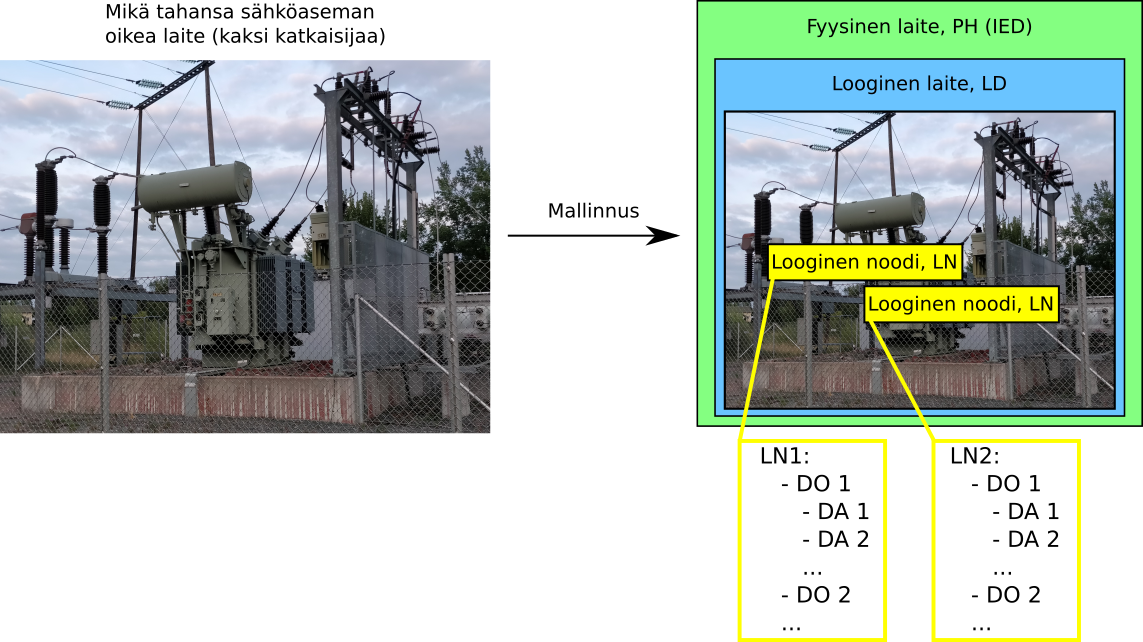
\includegraphics[width=1\textwidth]{pictures/substation-abstraction.png}
	\caption{Sähköaseman fyysisten laiteiden abstrahointi IEC 61850 -standardin käsitteillä (pohjautuu kuvaan \mbox{\cite[s.~17]{IEC61850-7-1}}).}
	\label{fig:substation-abstraction}
\end{figure}

IEC 61850 -standardin käsitteiden avulla sähköaseman laitteet ja funktiot voidaan esittää malleilla. Malleja voidaan käyttää IED-laitteiden konfiguroinnin määrittämiseen ja tietona, jotka voidaan siirtää verkon yli laitteelta toiselle. Jotta käsitteitä voidaan käyttää konfigurointiin ja kommunikointiin, standardi määrittää lisää tarkkuutta käsitteisiin ja kuinka niitä käytetään. MMS-protokollan kontekstissa fyysinen laite -käsite yksilöidään IP-osoitteella. Tämä käsite on olemassa standardissa, jotta oikea laite voidaan pitää abstraktina toteutettavasta tekniikasta. Muut käsitteet, eli looginen laite, looginen noodi, dataobjekti ja data-attribuutti määritellään standardissa luokilla tai tyypeillä. Kuvassa \ref{fig:iec61850-class-hierarchy} olevassa luokkakaaviossa on esitetty kuinka käsitteet muodostavat hierarkian toisistaan ja mistä standardin osasta käsitteen mallit löytyvät. Huomiona että dataobjektit ja data-attribuutit voivat viitata itseensä. Esimerkkinä dataobjekti voi sisältää myös alidataobjektin, joka taas sisältää data-attribuutteja. \mbox{\cite[s.~20--22]{IEC61850-7-2}}

\begin{figure}[ht!]
	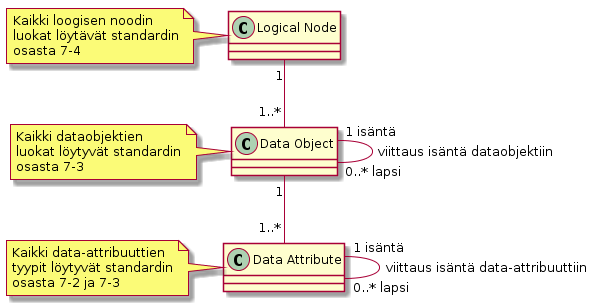
\includegraphics[width=0.8\textwidth]{pictures/iec61850-class-hierarchy.png}
	\caption{IEC 61850 -standardissa määritettyjen luokkien hierarkia (pohjautuu kuvaan \mbox{\cite[s.~17]{IEC61850-7-2}}).}
	\label{fig:iec61850-class-hierarchy}
\end{figure}

Looginen laite ja noodi yksilöidään nimillä, jotka ovat yksilöllisiä IED-laitteessa. Standardi asettaa rajoitteita nimeämiseen kuten pituuden. Looginen noodi esitetään IED-laitteella jonkin standardissa määritetyn luokan instanssina. Standardin osassa 7-4 määritellään valmiita luokkia käytettäväksi eri laitteiden esittämiseen. Esimerkiksi katkaisija on määritelty luokkaan tyypiltään \emph{XCBR} (engl. circuit breaker) \mbox{\cite[s.~105--106]{IEC61850-7-4}}. Sähköaseman insinööri, joka konfiguroi IED-laitteen, määrittää konfiguraatiotiedostossa, että kytketty katkaisija esitetään XCBR-luokan instanssina ja nimeää sen standardin ohjeiden mukaan. Näin IED-laite tietää mitä laitetta se esittää ja ohjaa. IED-laitteessa kaikki eri luokkien instanssit yksilöidään nimillä ja niitä käytetään, kun olioon viitataan esimerkiksi palvelukutsulla tai konfiguraatiolla. Looginen noodi koostui dataobjekteista. Standardissa dataobjektit ovat myös määritetty luokilla, joista tehdään instansseja. Loogisen noodin luokan tyyppi määrittää mitä dataobjektin luokista tehdään instansseja ja millä nimellä ne esitetään. Toisin sanoen, aseman insinööri voi valita käytettävän loogisen noodin instanssin nimen, mutta ei voi valita sen dataobjektin nimiä. Standardi määrittää dataobjektien luokkien tyypit standardissa osassa 7-3. Dataobjekti koostuu data-attribuuteista, kuten loogisen noodin luokka koostuu dataobjekteista. Dataobjektin luokka määrittää käytettävät data-attribuutit ja niiden nimet. Kuitenkaan tällä kertaa data-attribuutti ei välttämättä ole luokka. Data-attribuutit voivat olla primitiivisiä tyyppejä, kuten \emph{integer} ja \emph{float}. Ne voivat myös olla ns. \emph{rakennettuja data-attribuutteja} (engl. \emph{constructed attribute classes}), jotka pitävät sisällään tarkempia data-attribuutteja. Hyvä esimerkki on data-attribuutti nimeltään \emph{q}, jonka tyyppi on \emph{Quality}. Standardin mukaan tällä tyypillä on vielä aliattribuutteina mm. \emph{validity}, \emph{detailQual} jne \mbox{\cite[s.~11]{IEC61850-7-3}}. Tämä on esitetty kuvassa \ref{fig:iec61850-class-hierarchy} data-attribuutin itseensä viittauksella. Myös dataobjekti voi sisältää alidataobjekteja, jonka alla on taas omat data-attribuutit. Kappaleessa \ref{ch:luokkien-rakentuminen-instanseista} käydään tarkemmin läpi, kuinka luokkien hierarkia standardissa rakentuu. \mbox{\cite{IEC61850-1, IEC61850-7-1, IEC61850-7-2, IEC61850-7-3}}


\section{Loogisen noodin luokkien ja attribuuttien rakentuminen}
\label{ch:luokkien-rakentuminen-instanseista}
IEC 61850 -standardissa kaikki luokat määritellään taulukoilla, joissa on standardoitu kentän nimi, tyyppi, selitys ja onko se valinnainen. Tässä kappaleessa mennään syvemmälle luokkien määritykseen. Lisäksi esitetään esimerkkinä, kuinka standardin pohjalta tehty loogisen noodin instanssi ja sen alla olevat dataobjektit ja data-attribuutit rakentuvat. Esimerkissä käytetään kuvan \ref{fig:iec61850-data-modeling} rakennetta. 

Nimet ja luokkien instanssit konfiguroidaan IED-laitteelle XML-pohjaisella konfiguraatiotiedostolla. Tämä määritellään standardin osassa 6. Kuvassa \ref{fig:iec61850-data-modeling} fyysinen laite on IED-laite ja siihen verkossa viitataan IP-osoitteella 192.192.1.100. IED-laitteelle on konfiguroitu looginen laite nimeltä MyLD. Eri loogiset laitteet IED-laitteella yksilöi vain sen nimi. Loogisella laitteella on kaksi instanssia loogisen noodin luokista nimillä \emph{MMXU1} ja \emph{XCBR1}. MMXU1-instanssi on tyyppiä \emph{MMXU} (engl. measurement) \mbox{\cite[s.~57--58]{IEC61850-7-4}} ja XCBR1 on tyyppiä \emph{XCBR} (engl. circuit breaker). Kyseessä on siis vastaavasti mittaukseen liittyvä laite ja aikaisemmin mainittu linjan katkaisija. XCBR1 loogisella noodilla on dataobjekti nimeltään \emph{Pos} (engl. position), joka on tyyppiä \emph{DPC} (engl. controllable double point). Ja MMXU1 nimeltään \emph{TotW} (engl. total active power), joka on tyyppiä \emph{MV} (engl. measured value). Loogisilla noodeilla on määritetty enemmänkin dataobjekteja eri nimillä, mutta kuvassa \ref{fig:iec61850-data-modeling} on esitetty vain yhdet yksinkertaisuuden takia. Pos-dataobjektilla on data-attribuutit nimeltään \emph{stVal}, \emph{q} ja \emph{t}. Ja TotW-dataobjektilla on data-attribuutit \emph{mag}, \emph{q} ja \emph{t}. Esimerkin data-attribuutti q on tyyppiä Quality, jolla on alidata-attribuutteja ja attribuutti StVal on tyyppiä boolean. \mbox{\cite{IEC61850-7-3, IEC61850-7-4}}

\begin{figure}[ht!]
	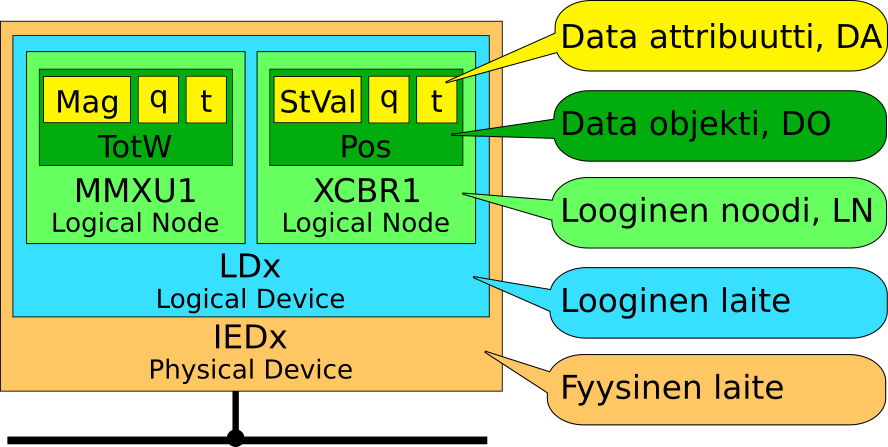
\includegraphics[width=1\textwidth]{pictures/iec61850-data-modeling.png}
	\caption{Standardin käsitteiden hierarkkinen rakenne ja niiden nimeämisen esimerkki (pohjautuu kuvaan \mbox{\cite[s.~24]{IEC61850-1}}).}
	\label{fig:iec61850-data-modeling}
\end{figure}

Standardissa osassa 7-4 on lista kaikista sen määrittämistä loogisen noodin luokista eri tarkoituksiin. Taulukossa \ref{tab:iec61850-xcbr-class-definition} on esitetty XCBR-luokan määritys. Taulukosta voi nähdä luokan instanssille määritetyt kenttien nimet ja viimeinen sarake M/O/C, kertoo, onko kenttä pakollinen (Mandatory, M), valinnainen (Optional, O), vai ehdollinen (Conditional, C). Taulukosta voi nähdä kuvan \ref{fig:iec61850-data-modeling} esimerkin XCBR1-instanssin dataobjektin nimeltä Pos ja sen tyypin DPC. Standardissa dataobjektien luokkia kutsutaan \emph{yleisiksi luokiksi} (engl. \emph{Common Data Class}, lyhennetään \emph{CDC}). Dataobjektin luokkia voidaan käyttää rakentamaan monta eri loogisen noodin luokkaa. Tämän takia dataobjektin luokkia standardissa kutsutaan nimellä \emph{yleiset luokat}. Dataobjektin luokkien on tarkoitus kerätä yhteen samaan asiaan liittyvät data-attribuutit. CDC-luokkien määritykset löytyvät standardin osasta 7-3 \mbox{\cite[s.~26]{IEC61850-1}}. Joillakin CDC-luokkien attribuutteina voi olla vielä muita CDC-luokkia. Tällöin standardissa puhutaan \emph{yleisistä aliluokista} (engl. \emph{sub data object}). Tämä esiteltiin myös aikaisemmin kuvassa \ref{fig:iec61850-class-hierarchy} olevalla dataobjektin itseensä viittauksella. Esimerkkinä tästä on CDC-luokka \emph{WYE}, jolla on attribuuttina \emph{phsA} niminen kenttä, joka on tyyppiä \emph{CMV}. CMV on CDC-luokka, jolla on taas omat data-attribuuttinsa. \mbox{\cite[s.~51,61]{IEC61850-7-2}} \mbox{\cite[s.~36]{IEC61850-7-3}}

\begin{table}[ht!]
	\caption{IEC 61850 -standardin katkaisijaluokan XCBR -määritys (pohjautuu taulukkoon \mbox{\cite[s.~105--106]{IEC61850-7-4}}).}
	\label{tab:iec61850-xcbr-class-definition}
	\begin{tabular}{l | l | l | l}
		\hline
		\textbf{Dataobjektin nimi} & \textbf{Englanniksi} & \textbf{CDC-luokka} & \textbf{M/O/C} \\
		\hline \hline
		\multicolumn{4}{l}{\textbf{Selitys}} \\
		\hline
		EEName & External equipment name plate & DPL & O \\
		\hline
		\multicolumn{4}{l}{\textbf{Tila informaatio}} \\
		\hline
		EEHealt & External equipment health & ENS & O \\
		LocKey & Local or remote key & SPS & O \\
		Loc & Local control behaviour & SPS & M \\
		OpCnt & Operation counter & INS & M \\
		CBOpCap & Circuit breaker operating capability & ENS & O \\
		POWCap & Point on wave switching capability & ENS & O \\
		MaxOpCap & Circuit breaker operating capability & INS & O \\
		Dsc & Discrepancy & SPS & O \\
		\hline
		\multicolumn{4}{l}{\textbf{Mitatut arvot}} \\
		\hline
		SumSwARs & Sum of switched amperes, resettable & BRC & O \\
		\hline
		\multicolumn{4}{l}{\textbf{Kontrollit}} \\
		\hline
		LocSta & Switching authority at station level & SPC & O \\
		Pos & Switch position & DPC & M \\
		BlkOpn & Block opening & SPC & M \\
		BlkCls & Block closing & SPC & M \\
		ChaMotEna & Charger motor enabled & SPC & O \\
		\hline
		\multicolumn{4}{l}{\textbf{Asetukset}} \\
		\hline
		CBTmms & Closing time of breaker & ING & O \\
		\hline
	\end{tabular}
\end{table}

Taulukossa \ref{tab:iec61850-DPC-class-definition} on DPC-luokan määritys. DPC-luokan instanssi esiintyy nimellä Pos ja on myös XCBR-luokan attribuutti. Taulukosta voi nähdä kuvan \ref{fig:iec61850-data-modeling} esimerkissä esitetyt data-attribuutit stVal, q ja t ja niiden tyypit. Attribuuttien tyyppejä on paljon enemmänkin ja lukija voi tarvittaessa tarkistaa kaikki tyypit standardista. Tällä periaatteella standardi rakentaa kaikki muutkin luokat hierarkkisesti. Määrityksien avulla voidaan selvittää mitä dataobjekteja looginen noodi sisältää, ja mitä data-attribuutteja dataobjekti sisältää. Taulukossa \ref{tab:iec61850-DPC-class-definition} on myös määritetty data-attribuuttien \emph{funktionaaliset rajoitteet} (engl. \emph{Functional Constraint}, lyhennetään \emph{FC}), sekä mahdolliset \emph{liipaisimet} (engl. \emph{trigger options}, lyhennetään \emph{TrgOp}). Funktionaaliset rajoitteet käsitellään tarkemmin kappaleessa \ref{ch:fc-and-dataset} ja liipaisimet kappaleessa \ref{ch:viestien-tilaus-ja-tilauksen-konfigurointi}.

\begin{table}[ht!]
	\caption{IEC 61850 -standardin DPC-luokan määritys ja instanssin nimi on Pos (pohjautuu taulukkoon \mbox{\cite[s.~44]{IEC61850-7-3}}).}
	\label{tab:iec61850-DPC-class-definition}
	\begin{tabular}{l | l | l | l}
		\hline
		\textbf{Data-attribuutin nimi} & \textbf{Tyyppi} & \textbf{FC} & \textbf{Liipaisin (TrgOp)} \\
		\hline
		\multicolumn{4}{l}{\textbf{Tila ja ohjaus}} \\
		\hline
		origin & Originator & ST &  \\
		ctlNum & INT8U & ST &  \\
		stVal & CODEC ENUM & ST & dchg \\
		q & Quality & ST & qchg \\
		t & TimeStamp & ST &  \\
		stSeld & BOOLEAN & ST & dchg \\
		opRcvd & BOOLEAN & OR & dchg \\
		opOk & BOOLEAN & OR & dchg \\
		tOpOk & TimeStamp & OR &  \\
		\hline
		\multicolumn{4}{l}{\textbf{Vaihtoehtoinen ja estäminen}} \\
		\hline
		subEna & BOOLEAN & SV &  \\
		subVal & CODED ENUM & SV &  \\
		subQ & Quality & SV &  \\
		subID & VISIBLE STRING64 & SV &  \\
		blkEna & BOOLEAN & BL &  \\
		\hline
		\multicolumn{4}{l}{\textbf{Asetukset, selitys ja laajennos}} \\
		\hline
		pulseConfig & PulseConfig & CF & dchg \\
		ctlModel & CtlModels & CF & dchg \\
		sboTimeOut & INT32U & CF & dchg \\
		sboClass & SboClassses & CF & dchg \\
		operTimeout & INT32U & CF & dchg \\
		d & VISIBLE STRING255 & DC &  \\
		dU & UNICODE STRING255 & DC &  \\
		cdcNs & VISIBLE STRING255 & EX &  \\
		cdcName & VISIBLE STRING255 & EX &  \\
		dataNs & VISIBLE STRING255 & EX &  \\
		\hline
	\end{tabular}
\end{table}

Kaikkien yllämainittujen luokkien kenttien määritysten lisäksi standardi määrittää palveluita jokaiselle luokkatyypille erikseen. Palvelut ovat abstrahoituja rajapintafunktioita, joille määritellään pyynnöt ja vastaukset. Standardin osa joka määrittää tekniikan toteutuksen, määrittää myös kuinka palvelut sillä toimivat. Tässä työssä esimerkkinä MMS-protokollan määritys, eli osa 8-1. Esimerkkinä palveluista kaikille dataobjekteille on mm. \emph{GetDataValues}, joka palauttaa kaikki dataobjektin attribuuttien arvot. \emph{SetDataValues} kirjoittaa annetut data-att\-ri\-buut\-ti\-en arvot. Ja \emph{GetDataDirectory} palauttaa kaikki data-att\-ri\-buut\-ti\-en viitteet kyseisessä dataobjektista. Näitä ja muita abstrahoituja malleja viitataan standardissa lyhenteellä \emph{ACSI} (engl. \emph{Abstract Communication Service Interface}). \mbox{\cite[s.~15, 45--46]{IEC61850-7-2}} \mbox{\cite[s.~26]{IEC61850-7-1}}


\section{Attribuuttien viittaus hierarkiassa}
IEC 61850 -standardi määrittää erilaisia palvelukutsuja eri luokkatyypeille. Palvelukutsuilla voidaan mm. asettaa ja lukea arvoja IED-laitteen hierarkiassa. Standardi määrittää viittausformaatin, joka mahdollistaa instanssien viittaamisen IED-laitteen hierarkiassa. Määritettyä viittausta käytetään palvelukutsujen yhteydessä määrittämään mitä instansseja kutsu koskee. Viitteen lisäksi aikaisemmin mainittu funktionaalinen rajoite kertoo mihin data-attribuutteihin kutsu kohdistuu. Funktionaalinen rajoite mahdollistaa monen instanssin viittaamisen hierarkiassa samalla kertaa. Seurauksena on, että yhdellä palvelukutsulla voidaan kirjoittaa tai lukea monta eri data-attribuuttia. Tämä tullaan käsittelemään tarkemmin kappaleessa \ref{ch:fc-and-dataset}. Kuvassa \ref{fig:iec61850-data-reference} on esitetty kuinka standardi määrittää viitteen muodostumisen loogisesta laitteesta data-attribuuttiin asti. \mbox{\cite[s.~625--626]{Mackiewicz2006}}

% \begin{figure}[ht!]
%	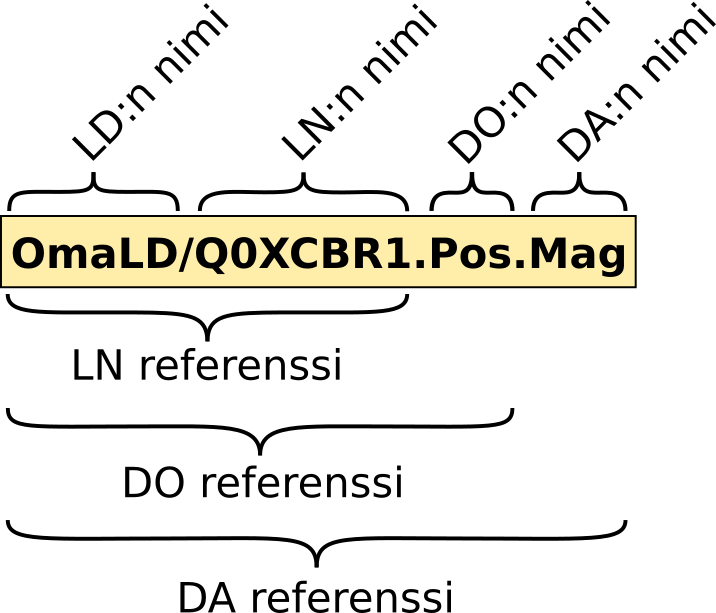
\includegraphics[width=0.5\textwidth]{pictures/iec61850-data-reference.png}
%	\caption{IEC 61850 -standardin määrittämä viitteen rakenne (pohjautuu kuvaan \mbox{\cite[s.~93]{IEC61850-7-1}}).}
%	\label{fig:iec61850-data-reference}
% \end{figure}

Viite muodostuu suoraan laitteessa olevien luokkien instanssien nimien ja hierarkian mukaan. Loogisen laitteen (\emph{LD}) ja loogisen noodin (\emph{LN}) erottimena käytetään \emph{kauttaviivaa} (/), ja muiden osien erottimena käytetään \emph{pistettä} (.). Loogisella laitteella on aseman insinöörin määrittämä alle 65-merkkinen nimi. Muuten loogisen laitteen nimeen standardi ei puutu. Loogisen noodin instanssin nimi koostuu alku-, keski- ja loppuosasta. Alkuosan voi insinööri itse päättää. Esimerkiksi kuvassa \ref{fig:iec61850-data-reference} loogisen noodin nimestä Q0 on alkuosa. Nimen täytyy alkaa kirjaimella, mutta se voi sisältää myös numeroita. Keskiosan täytyy olla loogisen luokan nimi, josta instanssi on tehty. Tässä tapauksessa jo aikaisemmin mainittu katkaisijan luokka, XCBR. Tämä osuus on aina 4 kirjainta pitkä ja aina isoilla kirjaimilla. Loppuosa on instanssin numeerinen arvo, joka ei sisällä kirjaimia. Insinööri voi itse päättää loppuosan, jonka ei tarvitse välttämättä olla juokseva numero. Esimerkiksi kuvassa \ref{fig:iec61850-data-reference} loogisen noodin nimen loppuosa on 1. 
Alku- ja loppuosan yhteenlaskettu merkkien pituus täytyy olla alle 13 merkkiä, eli koko loogisen noodin nimen pituus voi olla maksimissaan 17 merkkiä. Dataobjektien (\emph{DO}) ja attribuuttien (\emph{DA}) niminä käytetään standardin määrittämiä nimiä, jotka määritetään niitä vastaavissa luokissa osissa 7-3 ja 7-4 (katso taulukot \ref{tab:iec61850-xcbr-class-definition} ja \ref{tab:iec61850-DPC-class-definition}). Riippuen viittauksesta, näistä muodostuu loogisen noodin viite, dataobjektin viite ja data-attribuutin viite. Dataobjekti voi pitää sisällään toisen dataobjektin kuten aikaisemmin kuvassa \ref{fig:iec61850-class-hierarchy} esitettiin. Viittausta jatketaan liittämällä instanssien nimiä toisiinsa pisteellä aina data-attribuuttiin asti. Samoin toimitaan, kun data-attribuutti on tyypiltään rakennettu tyyppi, kuten Quality, jolla on alidata-attribuutteja. \mbox{\cite[s.~181--182]{IEC61850-7-2}} \mbox{\cite[s.~93--95]{IEC61850-7-1}}

Standardissa määritetään kaksi näkyvyysaluetta (engl. scope) viittaukselle, jotka ovat palvelin- ja looginen laite -näkyvyysalueet. Palvelin tarkoittaa tässä yhteydessä verkkoon kytkettyä laitetta, eli IED-laitetta. Palvelimen näkyvyysalueelle viitataan ottamalla viittauksesta pois loogisen laitteen nimi. Eli kuvassa \ref{fig:iec61850-data-reference} viittaus tulisi muotoon /Q0XCBR1"".""Pos"".""stVal. Edellä mainittua viittausta käytetään silloin, kun loogisen noodin instanssi sijaitsee loogisen laitteen ulkopuolella, mutta kuitenkin palvelimella. Loogisen laitteen näkyvyysalueessa viittaus sisältää loogisen laitteen nimen ennen kauttaviivaa, toisin kuin palvelimen näkyvyysalueessa. Esimerkiksi kuvassa \ref{fig:iec61850-data-reference} oleva viittaus OmaLD""/""Q0XCBR1"".""Pos"".""stVal. Loogisen laitteen näkyvyysaluetta käytetään silloin kun loogisen noodin instanssi sijaitsee loogisen laitteen sisällä sen hierarkiassa. Tässä työssä jatkossa käytetään pelkästään loogisen laitteen -näkyvyysaluetta. \mbox{\cite[s.~183]{IEC61850-7-2}}

Standardi määrittää viittausten maksimipituuden. Pituusmääritykset ovat voimassa kummallekin edellä mainitulle näkyvyysalueelle. Ennen kauttaviivaa saa olla maksimissaan 64 merkkiä. Tämän jälkeen kauttaviiva, josta seuraa uudelleen maksimissaan 64 merkkiä. Eli koko viittauksen maksimipituus saa olla enintään 129 merkkiä, kauttaviiva mukaan lukien. \mbox{\cite[s.~24,183]{IEC61850-7-2}}


\section{Attribuuttien funktionaalinen rajoite ja niistä muodostetut datajoukot}
\label{ch:fc-and-dataset}
Standardin CDC-luokat määrittävät käytettävät data-attribuutit (katso taulukko \ref{tab:iec61850-DPC-class-definition}). Nämä luokat määrittävät myös jokaiselle data-attribuutille aikaisemmin mainitun \emph{funktionaalisen rajoitteen} (engl. \emph{functional constraint}, lyhennetään \emph{FC}). Funktionaalinen rajoite kuvaa attribuutin käyttötarkoitusta, ja sen mitä palveluita attribuuttiin voidaan käyttää. Esimerkiksi kaikilla attribuuteilla, jotka liittyvät laitteen tilaan on funktionaalinen rajoite \emph{ST} (engl. \emph{status information}). Standardi määrittää paljon erilaisia funktionaalisia rajoitteita, jotka ovat kaikki kahden ison kirjaimen yhdistelmiä. Taulukossa \ref{tab:iec61850-functional-constraints} on esitetty joitain tärkeimpiä funktionaalisia rajoitteita. Funktionaalinen rajoite määrittää myös, onko attribuutti kirjoitettava tai luettava. \cite[s.~53--55]{IEC61850-7-2}

\begin{table}[ht!]
	\caption{Osa IEC 61850 -standardin määrittämistä funktionaalisista rajoitteista, lyhennetään FC (ote taulukosta \mbox{\cite[s.~54]{IEC61850-7-2}}).}
	\label{tab:iec61850-functional-constraints}
	\begin{tabular}{l | l | l | l}
		\hline
		\textbf{Lyhenne} & \textbf{Selite} & \textbf{Luettava} & \textbf{Kirjoitettava} \\
		\hline \hline
		ST & Laitteen tilatieto (status) & Kyllä & Ei \\
		MX & Mittaustieto (measurands) & Kyllä & Ei \\
		CF & Laitteen asetusarvo (configuration) & Kyllä & Kyllä \\
		DC & Selitystieto (description) & Kyllä & Kyllä \\
		\hline
	\end{tabular}
\end{table}

Funktionaalista rajoitetta käytetään IED-laitteelle tehdyssä kutsussa viitteen kanssa rajoittamaan mitä data-attribuutteja tehty kutsu koskee. Tästä tulee nimi funktionaalinen rajoite. Funktionaalinen rajoite on pakollinen tieto kutsuissa, jotka lukevat tai kirjoittavat arvoja. Seuraavaksi esitetään esimerkki, kuinka yhdellä kutsulla viitataan moneen data-attribuuttiin. Esimerkkinä otetaan kuvassa \ref{fig:iec61850-data-reference} olevasta viitteestä osa, joka viittaa dataobjektiin. Eli OmaLD/Q0XCBR1.Pos, jolloin viite on DO-viite. Kutsun vaikutusalue on aina hierarkiassa alaspäin. Eli nyt viitteellä viitataan Pos-dataobjektin kaikkiin alla oleviin data-attribuutteihin. Katso taulukko \ref{tab:iec61850-DPC-class-definition}, jossa on esitetty kaikki Pos-dataobjektin alla olevat data-attribuutit. Huomiona, jos viittauksen alla olisi alidataobjekteja, niidenkin data-attribuutit kuuluisivat viittauksen piiriin. Viittauksen vaikutuksen voi siis ajatella jatkuvan viittauskohdasta alaspäin hierarkiassa kaikkiin ali-instansseihin. Funktionaalista rajoitetta käytetään rajoittamaan/suodattamaan kaikista viitatuista data-attribuuteista ne, jotka halutaan kirjoittaa tai lukea. Esimerkkinä jos kutsuun viitteellä OmaLD/Q0XCBR1.Pos lisättäisiin funktionaalinen rajoite ST, rajoitettaisiin kutsu koskemaan Pos-dataobjektin alidata-attribuuteista vain niitä attribuutteja, joilla on funktionaalinen rajoite ST. Taulukossa \ref{tab:fc-usage-example} on esitetty esimerkkinä ne data-attribuutit, joihin kutsu viittaisi. Taulukon attribuutit ovat samat kuin Pos-dataobjektin attribuutit taulukossa \ref{tab:iec61850-DPC-class-definition}. Eli taulukon \ref{tab:fc-usage-example} mukaan, attribuutit olisivat origin, ctlNum, stVal, q, t ja stSeld. Muut data-attribuutit suodatetaan pois kutsun vaikutuksesta. Sama suodatus tapahtuu hierarkiassa alaspäin kaikille alidataobjekteille ja alidata-attribuuteille. Esimerkissä olevat attribuutit voisi vain lukea, ei kirjoittaa. Tämä sen takia, että taulukon \ref{tab:iec61850-functional-constraints} mukaan funktionaalinen rajoite ST sallii vain lukemisen. IEC 61850 -standardissa määritetään funktionaalinen rajoite XX, joka on sama kuin mikä tahansa muu funktionaalinen rajoite. Kuitenkin standardin osassa 8-1, joka tekee toteutuksen MMS-protokollalle, tämä ei ole tuettu toiminnallisuus. Eli toisin sanoen, jos MMS-protokollan kanssa halutaan lukea kaikki yhden dataobjektin data-attribuutit, joudutaan tekemään kutsu jokaista dataobjektin funktionaalista rajoitetta kohti. MMS-protokollan määrityksessä ei määritetä kutsua, jolla pystyisi lukemaan vain yhden dataobjektin kaikki data-attribuutit. Monta erillistä kutsua tarvitaan. \mbox{\cite{IEC61850-7-2}}

\begin{table}[ht!]
	\caption{Pos-dataobjektista viitteellä OmaLD/Q0XCBR1.Pos ja funktionaalisella rajoitteella ST viitatut data-attribuutit.}
	\label{tab:fc-usage-example}
	\begin{tabular}{l | l | l }
		\hline
		\textbf{Data-attribuutin nimi} & \textbf{FC} & \textbf{Viittaa} \\
		\hline \hline
		origin & ST & kyllä \\
		ctlNum & ST & kyllä \\
		stVal & ST & kyllä \\
		q & ST & kyllä \\
		t & ST & kyllä \\
		stSeld & ST & kyllä \\
		opRcvd & OR & ei \\
		opOk & OR & ei \\
		tOpOk & OR & ei \\
		subEna & SV & ei \\
		subVal & SV & ei \\
		subQ & SV & ei \\
		subID & SV & ei \\
		blkEna & BL & ei \\
		pulseConfig & CF & ei \\
		ctlModel & CF & ei \\
		sboTimeOut & CF & ei \\
		sboClass & CF & ei \\
		operTimeout & CF & ei \\
		d & DC & ei \\
		dU & DC & ei \\
		cdcNs & EX & ei \\
		cdcName & EX & ei \\
		dataNs & EX & ei \\
		\hline
	\end{tabular}
\end{table}

Viittauksen ja funktionaalisen rajoitteen avulla siis suodatetaan hierarkiassa alaspäin olevia dataobjekteja ja data-attribuutteja. IEC 61850 -standardissa on määritelty nimitykset käytettäväksi, kun jotakin viittausta suodatetaan funktionaalisella rajoitteella. Nämä ovat \emph{FCD} (engl. \emph{Functional Constrained Data}) ja \emph{FCDA} (engl. \emph{Functional Constrained Data Attribute}). Nämä nimitykset ovat standardissa vain käsite ja niitä käytetään, kun asiasta mainitaan. Taulukossa \ref{tab:fcd-ja-fcda} on esitetty viittauksia eri tyyppisiin instansseihin funktionaalisella rajoitteella. Taulukosta selviää, onko viitattu instanssi dataobjekti (DO) vai data-attribuutti (DA). Myös sen instanssin tyyppi ja käytetty nimitys viittaukselle FCD tai FCDA. Viitteestä käytetään FCD-nimitystä vain silloin kun hierarkian ensimmäistä dataobjekti rajoitetaan funktionaalisesti. FCDA-nimitys on käytössä kaikille muille viittauksille hierarkiassa alaspäin, joita rajoitetaan funktionaalisesti. Huomaa taulukossa \ref{tab:fcd-ja-fcda} viittaus OmaLD/MMXU1.PhV.phsA, joka viittaa PhV dataobjektin alidataobjektiin. Tämä on FCDA-viittaus, vaikka kyseessä onkin dataobjekti. Ainoa ero FCD:n ja FCDA:n viittausten välillä on vain se, että FCD-viittaus on aina vain hierarkian ensimmäiseen dataobjektiin ja FCDA-viittaus siitä alaspäin hierarkiassa. \mbox{\cite[s.~55]{IEC61850-7-2}} \mbox{\cite[s.~63]{IEC61850-8-1}}

\begin{table}[ht!]
	\caption{Viitteen nimeäminen lyhenteellä funktionaalisen rajoitteen kanssa.}
	\label{tab:fcd-ja-fcda}
	\begin{tabular}{l | l | l | l | l}
		\hline
		\textbf{FC} & \textbf{Viite} & \textbf{Instanssi} & \textbf{Tyyppi} & \textbf{Nimitys} \\
		\hline \hline
		ST & OmaLD/XCBR1.Pos & DO & DPC & FCD \\
		ST & OmaLD/XCBR1.Pos.t & DA & TimeStamp & FCDA \\
		ST & OmaLD/XCBR1.Pos.ctlNum & DA & INT8U & FCDA \\
		MX & OmaLD/MMXU1.PhV & DO & WYE & FCD \\
		MX & OmaLD/MMXU1.PhV.phsA & DO & CMV & FCDA \\
		MX & OmaLD/MMXU1.PhV.phsA.t & DA & TimeStamp & FCDA \\
		\hline
	\end{tabular}
\end{table}

Funktionaalista rajoitetta käytetään viitteen kanssa suodattamaan viitatusta kohdasta alaspäin kaikki data-attribuutit. Tätä toiminnallisuutta käytetään hyväksi, kun tehdään kirjoittavia tai lukevia kutsuja ja rajoitetaan kutsulla vaikutettavia data-attribuutteja. Tätä samaa mekanismia käytetään hyväksi, kun IED-laitteeseen määritellään \emph{datajoukkoja}. IEC 61850 -standardissa datajoukko koostuu joukosta IED-laitteessa olemassa olevista data-attribuuteista. Datajoukko on tapa koostaa yhteen kiinnostavat data-attribuutit IED-laitteelta. Datajoukko nimetään ja sijoitetaan IED-laitteen hierarkiaan. Näin siihen voidaan viitata kutsuilla, kuten mihin tahansa muuhun hierarkian instanssiin. Datajoukot IED-laitteelle rakennetaan käyttämällä FCD- ja FCDA-viitteitä. Datajoukko koostuu siis joukosta FCD- ja FCDA -viitteitä. Jokaisella viitteellä on jokin funktionaalinen rajoite, joka suodattaa viitteen alla olevat attribuutit ja sisällyttää ne kyseiseen datajoukkoon. Esimerkkinä datajoukon rakentamisesta taulukon \ref{tab:fcd-ja-fcda} viitteet. Näistä viitteistä olisi mahdollista rakentaa standardin mukainen datajoukko, nimetä se nimellä Testi1, ja lisätä IED-laitteen hierarkiaan kohtaan OmaLD/LLN0.Testi1. Nyt datajoukkoon pystyy viittaamaan ja sen arvoja lukemaan. Jotta datajoukko saadaan näin tehtyä, tieto tästä täytyy lisätä IED-laitteen asetustiedostoon. Datajoukkoja IED-laitteessa käytetään muodostamaan joukkoja tärkeistä data-attribuuteista, joita voidaan esimerkiksi lukea ja kirjoittaa yhdellä kutsulla. Datajoukkoja käytetään myös tilattavien \emph{viestien sisältönä}. Viestejä voi standardin mukaan tilata vain datajoukoista olevista data-attribuuteista. \mbox{\cite[s.~61--68]{IEC61850-7-2}}


\section{Viestien tilaus ja tilauksen konfigurointi}
\label{ch:viestien-tilaus-ja-tilauksen-konfigurointi}
IEC 61850 -standardi määrittää, kuinka IED-laitteen ulkopuolinen ohjelma voi tilata kiinnostavien data-attribuuttien arvoja verkon yli. Viesti voidaan esimerkiksi lähettää tilaajalle, kun mitatun jännitteen arvo muuttuu. Kyseessä on tilaaja-julkaisija-arkkitehtuurimalli, jossa ulkopuolinen ohjelma on tilaaja ja IED-laite julkaisuja. Standardi määrittää, että viestejä voidaan tilata vain datajoukoissa viitatuilla data-attribuuteilta. Viestien lähetyksen tiheys riippuu siitä, kuinka tilauksen yhteydessä tilaaja asettaa \emph{liipaisimet}. Standardissa määritellään käytettäväksi erilaisia liipaisimia, joilla tilaaja voi muokata millä ehdoilla viesti lähetetään. Standardissa on myös määritetty mekanismit, joilla tilaajaa voi pyytää kaikki arvot kerralla tai tilata jaksottaisia viestejä tietyn aikavälein. \mbox{\cite{IEC61850-7-1}}

Standardissa määritetään luokka, jonka tehtävä on hoitaa tilausta ja sen asetuksia. Tässä kappaleessa käydään läpi luokan yleistä toiminnallisuutta. Kappaleessa \ref{ch:rcb-toiminta} käsitellään luokan attribuutteja ja toimintaa tarkemmin. Niin kuin muutkin luokat standardissa, siitä tehdään instanssi, sille annetaan yksilöivä nimi ja se lisätään IED-laitteen hierarkiaan. Nämä määritellään IED-laitteen asetustiedostossa, kuten kaikki muutkin instanssit. Yksilöivän nimen avulla tilaaja voi viitata kutsulla instanssiin, muuttaa luokan asetuksia ja aloittaa tilauksen. Nämä luokat standardissa ovat \emph{puskuroitu viestintäluokka} (engl. \emph{Buffered Report Control Block}, lyhennetään \emph{BRCB}) ja \emph{ei puskuroitu luokka} (engl. \emph{Unbuffered Report Control Block}, lyhennetään \emph{URCB}). Tekstissä kumpaakin luokkaan viitatessa käytetään lyhennettä \emph{RCB}. Ainoa ero luokkien toiminnan välillä on, että BRCB puskuroi viestejä jonkin aikaa yhteyden katkettua. Yhteyden palautuessa, se lähettää puskuroidut viestit järjestyksessä asiakkaalle. BRCB takaa viestien järjestyksen ja saatavuuden. URCB lähettää viestejä asiakkaalle ilman puskurointia ja viestit menetetään yhteyden katketessa. Standardissa määritetään, että yksi RCB-instanssi voi palvella vain yhtä tilaaja kerrallaan. IED-laitteeseen täytyy määrittää instansseja sen tilaajien määrän mukaan. \mbox{\cite[s.~93]{IEC61850-7-2}}

Sekvenssikaaviossa \ref{fig:iec61850-brcb-communication} on esitetty tilaajan ja IED-laitteella olevan BRCB-instanssin välinen viestien tilauksen prosessi. Kaaviossa ensin asiakas tilaa puskuroidun BRCB-ins\-tans\-sin (kohdat 1--2). Ensimmäisessä kutsussa tilaaja kirjoittaa BRCB-luokan arvot, kuten käytettävät liipaisimet jne. Kutsussa tilaajan on merkittävä RCB-ins\-tans\-si varatuksi, jotta tilaus käynnistyy. BRCB aloittaa viestien julkaisun tilaajalle määritettyjen ehtojen mukaan (kohdat 3--4). Jos tilaajan ja IED-laitteen välinen yhteys katkeaa, BRCB-instanssi puskuroi viestejä johonkin järkevään rajaan asti. Kun yhteys tilaajaan palaa, BRCB lähettää viestit järjestyksessä tilaajalle alkaen ensin puskurista (kohdat 5--7). Tilaaja voi lopettaa tilauksen ja instanssin varauksen merkitsemällä sen taas vapaaksi (kohdat 8--9). \mbox{\cite[s.~41--42]{IEC61850-7-1}}

\begin{figure}[ht!]
	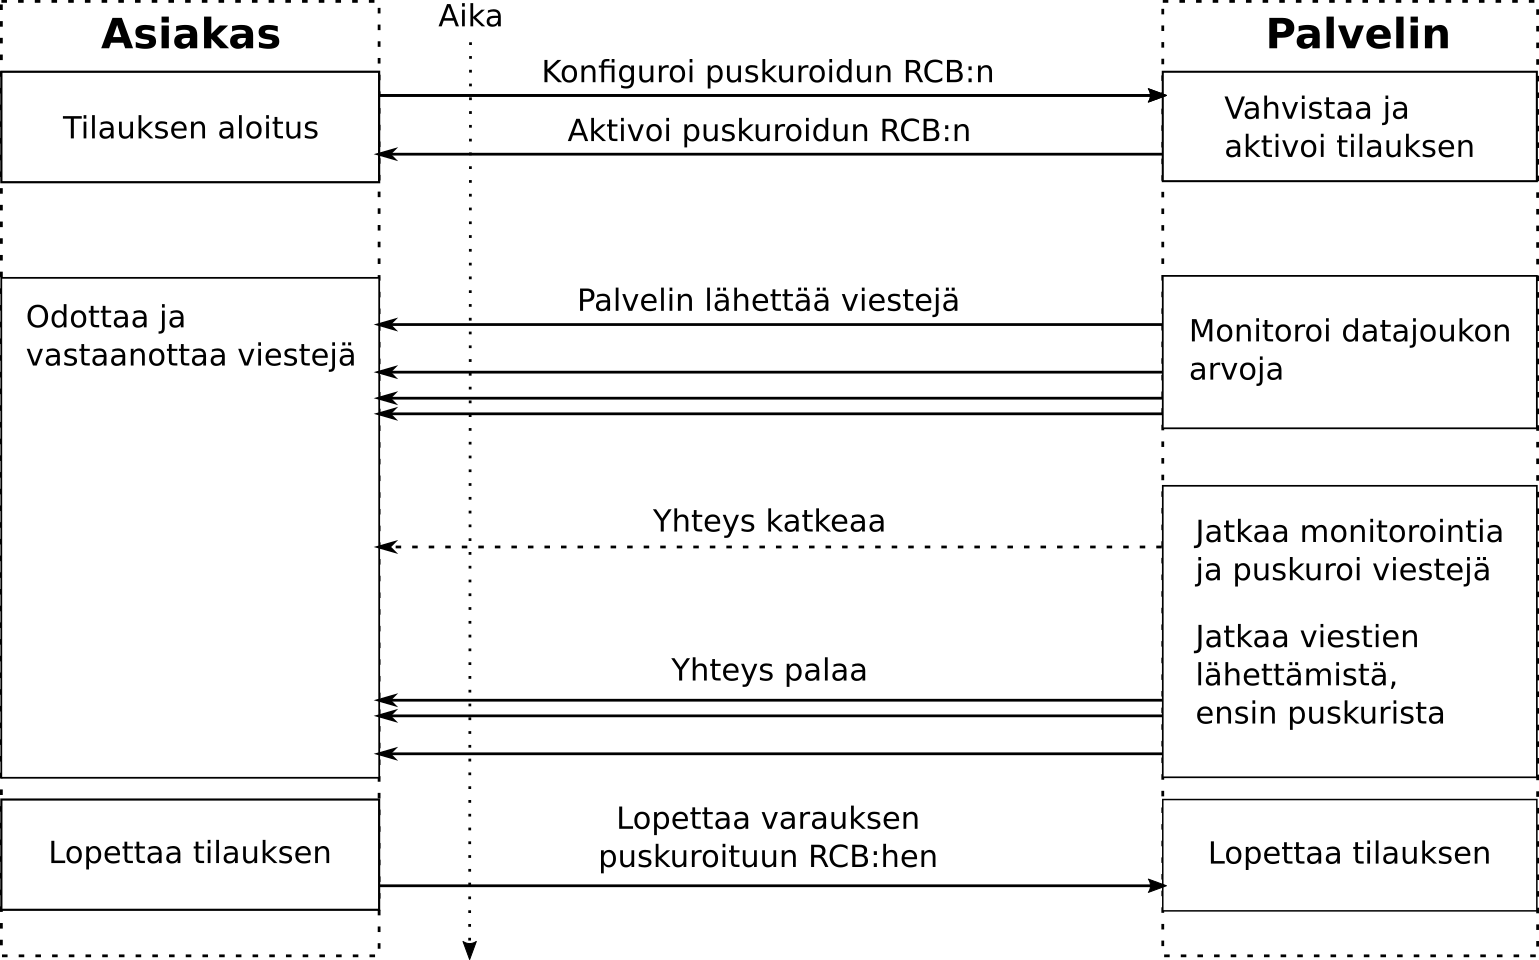
\includegraphics[width=0.5\textwidth]{pictures/iec61850-brcb-communication.png}
	\caption{Puskuroitu viestien tilausprosessi tilaajan ja IED-laitteella olevan BRCB-instanssin välillä (pohjautuu kuvaan \mbox{\cite[s.~42]{IEC61850-7-1}}).}
	\label{fig:iec61850-brcb-communication}
\end{figure}

Standardissa määritetään, että viestejä voidaan tilata vain datajoukoista. IED-laitteen asetustiedostossa täytyy myös määrittää mitä datajoukkoa RCB-instanssi käyttää. Tämän jälkeen instanssi tarkkailee datajoukon attribuuttien muutoksia ja lähettää viestin, jos tilaajan asettama liipaisin täsmää. Koska yksi RCB voi palvella vain yhtä tilaajaa kerrallaan, täytyy samaan datajoukkoon viitata monella eri RCB-instanssilla. Näin monta eri tilaajaa saavat viestin samasta tapahtumasta. \mbox{\cite[s.~93]{IEC61850-7-2}}

Standardissa on määritetty seuraavat liipaisimet data-attribuuteille, joita RCB tarkkailee ja reagoi niihin:
\begin{itemize}
	\item \emph{datan muutos} (engl. \emph{data change}, standardissa lyhenne \emph{dchg}),
	\item \emph{laadun muutos} (engl. \emph{quality change}, standardissa lyhenne \emph{qchg}), ja
	\item \emph{datan päivitys} (engl. \emph{data update}, standardissa lyhenne \emph{dupd}).
\end{itemize}

Standardin luokissa on määritetty mitä liipaisimia data-attribuutti tukee. Esimerkkinä aikaisemmin mainittu DPC-luo\-kan määritys taulukossa \ref{tab:iec61850-DPC-class-definition}, jossa TrgOp-sarake kertoo attribuutin liipaisimen. Datan muutos ja päivitys liipaisimien ero on, että datan päivitys liipaisee tapahtuman, vaikka attribuutin uusi arvo olisi sama. Datan muutos ei liipaise tapahtumaa, jos uusi arvo on sama kuin edellinen arvo. Laadun muutos liipaisin tarkoittaa, että data-attribuuttiin liitetty laatuarvo muuttui. Laatuarvo kertoo tilaajalle ja arvojen lukijalle, voiko attribuuttien arvoihin luottaa. Laatuarvo on tyyppiä Quality ja tästä voi tarvittaessa lukea enemmän standardista. \mbox{\cite[s.~90]{IEC61850-7-1}}


\section{Raportointi-luokan määritys ja toiminta}
\label{ch:rcb-toiminta}
BRCB-luokalla on erilaisia attribuutteja, joita tilaaja voi kirjoittaa ja lukea ennen tilauksen aloittamista. BRCB ja URCB -luokat eivät eroa paljon attribuuteilla toisistaan, joten tässä kappaleessa keskitytään vain BRCB-luokan toimintaan. Tarkka määritys luokkien eroista löytyy standardin osasta 7-2. Taulukossa \ref{tab:iec61850-brcb-class-definition} on esitetty standardin määrittämän BRCB-luokan attribuutit, attribuutin nimi englanniksi ja sen selite. Taulukossa ei ole esitetty attribuuttien tyyppejä, koska ne voi lukija tarvittaessa tarkemmin lukea standardin omasta määrityksestä. Lisäksi tässä kappaleessa käydään läpi luokan attribuuttien toimintaa pääpiirteittäin ja loput tiedot lukija voi tarkistaa standardista.

\begin{table}[ht!]
	\caption{BRCB-luokan määritetyt attribuutit ja niiden selitteet (pohjautuu taulukkoon \mbox{\cite[s.~94]{IEC61850-7-2}}).}
	\label{tab:iec61850-brcb-class-definition}
	\begin{tabular}{l | l | l}
		\hline
		\textbf{Attribuutti} & \textbf{Englanniksi} & \textbf{Selite} \\
		\hline \hline
		BRCBName & BRCB name & Objektin nimi \\
		&\\
		BRCBRef & BRCB reference & Objektin viite \\
		&\\
		RptID & Report identifier & \parbox[t]{7.5cm}{RCB-instanssin yksilöivä id lähetettyihin viesteihin, asiakas voi asettaa} \\
		&\\
		RptEna & Report enable & Varaa RCB:n ja aloittaa viestien lähetyksen \\
		&\\
		DatSet & Data set reference & Tarkkailtavan datajoukon viite \\
		&\\
		ConfRev & Configuration revision & \parbox[t]{7.5cm}{Juokseva konfiguraation numerointi, muutos kasvattaa numerointia} \\
		&\\
		OptFlds & Optional fields & Mitä valinnaisia kenttiä viestiin lisätään \\
		&\\
		BufTm & Buffer time & \parbox[t]{7.5cm}{Puskurointiaika, ennen viestin lähetystä. Tänä aikana tapahtuvat liipaisut yhdistetään samaan viestiin} \\
		&\\
		SqNum & Sequence number & Juokseva lähetetyn viestin numerointi \\
		&\\
		TrgOps & Trigger options & Millä liipaisimilla viesti lähetetään \\
		&\\
		IntgPd & Integrity period & \parbox[t]{7.5cm}{Periodisen viestien väli millisekunteina, arvolla 0 ei käytössä} \\
		&\\
		GI & General-interrogation & \parbox[t]{7.5cm}{Käynnistää yleiskyselyn, joka sisältää kaikki datajoukon attribuutit seuraavaan viestiin} \\
		&\\
		PurgeBuf & Purge buffer & Puhdistaa lähettämättömät viestit puskurista \\
		&\\
		EntryID & Entry identifier & \parbox[t]{7.5cm}{Puskurissa olevan viimeisimmän viestin id. Arvo 0 tarkoittaa tyhjää puskuria} \\
		&\\
		TimeOfEntry & Time of entry & \parbox[t]{7.5cm}{Puskurissa olevan viimeisimmän viestin aikaleima} \\
		&\\
		ResvTms & Reservation time & \parbox[t]{7.5cm}{Instanssin varausaika sekunteina kun yhteys katkeaa, arvo -1 tarkoittaa konfiguraation aikaista varausta ja 0 että ei varausta} \\
		&\\
		Owner & Owner & \parbox[t]{7.5cm}{Yksilöi varaavan asiakkaan, yleensä IP-osoite tai IED-laitteen nimi. Arvo 0 että RCB on vapaa tai ei omistajaa} \\
		\hline
	\end{tabular}
\end{table}

Tilaaja voi vapaasti kirjoittaa ja lukea RCB-instanssin arvoja monella peräkkäisellä kutsulla ennen tilauksen aloittamista. Tärkein attribuutti on boolean tyyppinen \emph{RptEna}. Kirjoittamalla sen arvoon tosi tilaaja aloittaa tilauksen ja varaa instanssin itselleen. Tilaaja voi edelleen lukea ja kirjoittaa sen arvoja tilauksen ollessa päällä, mutta rajoitetusti. Joidenkin arvojen kirjoitus pitää tapahtua ennen tilausta tai samassa kutsussa, kun RtpEna asetetaan arvoon tosi. Tilaaja lopettaa tilauksen, jos yhteys on poikki tarpeeksi kauan tai RptEna kirjoitetaan arvoon epätosi. \mbox{\cite[s.~95--97]{IEC61850-7-2}}

RCB-luokan TrgOps-attribuutti on binääritietue, jossa yksittäinen bitti ilmaisee mikä liipaisin aiheuttaa viestin lähettämisen. Tällä attribuutilla tilaaja voi päättää mitä liipaisimia hän haluaa käyttää. TrgOps sisältää seuraavat liipaisimet:
\begin{itemize}
	\item \emph{datan muutos} (engl. \emph{data change}, standardissa lyhenne \emph{dchg}),
	\item \emph{laadun muutos} (engl. \emph{quality change}, standardissa lyhenne \emph{qchg}),
	\item \emph{datan päivitys} (engl. \emph{data update}, standardissa lyhenne \emph{dupd}),
	\item \emph{yleinen kysely} (engl. \emph{general-interrogation}, standardissa lyhenne \emph{GI}), ja 
	\item \emph{jatkuva viestintä väliajoin} (engl. \emph{integrity}) \cite[s.~100]{IEC61850-7-2}.
\end{itemize}

Kolme ensimmäistä liipaisinta dchg, qchg ja dupd ovat aikaisemmin kappaleessa \ref{ch:viestien-tilaus-ja-tilauksen-konfigurointi} määritettyjen data-attribuuttien liipaisimia. Asiakas voi tilata viestejä esimerkiksi vain datan muutoksista. RCB-luokka määrittää data-attribuuttien liipaisimien lisäksi vielä kaksi liipaisinta lisää, yleinen kysely ja jatkuva viestintä väliajoin. Yleinen kysely on viesti, johon RCB sisällyttää kaikki datajoukon attribuutit. Asiakas voi liipaista sen asettamalla GI-attribuutin arvoksi tosi ja TrgOps-attribuutissa liipaisin on päällä. Tällöin RCB käynnistää viestin generoinnin ja lähettää sen asiakkaalle. Jos liipaisin ei ole päällä TrgOps-attribuutissa ja GI arvoksi asetetaan tosi, RCB ei generoi viestiä. Viestin lähetyksen jälkeen RCB itse asettaa GI:n arvoksi epätosi. Jatkuva viestintä -liipaisin on jatkuvaa viestin lähettämistä tilaajalle asetetun väliajoin, johon sisältyy kaikki datajoukon attribuutit. Toiminnon saa päälle, kun asiakas asettaa RCB-luokassa attribuutit \emph{IntgPd} arvoksi muu kuin 0, ja TrgOps-attribuutin arvossa kyseinen liipaisin on päällä. IntgPd-attribuutti kertoo minkä väliajoin viesti generoidaan ja lähetetään asiakkaalle. Jos IntgPd arvo on muu kuin 0 ja TrgOps-attribuutissa liipaisin ei ole päällä, ei viestiä generoida ja lähetetä asiakkaalle väliajoin. \mbox{\cite[s.~100--102]{IEC61850-7-2}}

RCB-luokan \emph{OptFlds}-attribuutin avulla asiakas voi valita mitä vaihtoehtoisia kenttiä viestiin sisällytetään. OptFlds on binääritietue niin kuin ja TrgOps. Taulukossa \ref{tab:iec61850-optional-fields-definition} on esitetty sen asetettavat arvot. Taulukon yksittäinen kenttä vastaa OptFlds-arvon yhtä bittiä. Bittien järjestys määräytyy tekniikalle toteutuksen perusteella. Esimerkiksi MMS-protokolla. Taulukon arvoilla tilaaja voi määrittää mitä lisätietoa viestiin sisällytetään. Esimerkiksi asettamalla reason-for-inclusion bitin päälle, liitetään viestin arvon yhteyteen tieto, miksi tämä viestiin sisällytettiin. Viestin rakennetta ja kuinka OptFlds-attribuutin arvoilla sen sisältöön voi vaikuttaa käydään läpi tarkemmin kappaleessa \ref{ch:viestin-rakenne}. \mbox{\cite[s.~98]{IEC61850-7-2}}

\begin{table}[ht!]
	\caption{RCB-luokan OptFlds-attribuutin arvot ja niiden selitteet.}
	\label{tab:iec61850-optional-fields-definition}
	\begin{tabular}{l | l}
		\hline
		\textbf{Arvo} & \textbf{Selite} \\
		\hline \hline
		sequence-number & Jos tosi, sisällytä RCB-luokan attribuutti SqNum viestiin \\
		report-time-stamp & Jos tosi, sisällytä RCB-luokan attribuutti TimeOfEntry viestiin \\
		reason-for-inclusion & Jos tosi, sisällytä syy miksi arvo(t) sisällytettiin viestiin \\
		data-set-name & Jos tosi, sisällytä RCB-luokan attribuutti DatSet viestiin \\
		data-reference & \parbox[t]{10cm}{Jos tosi, sisällytä datajoukon liipaisseen kohdan rakentamiseen käytetty FCD- tai FCDA-viite viestiin} \\
		buffer-overflow & \parbox[t]{10cm}{Jos tosi, sisällytä viestiin tieto onko puskuri vuotanut yli kentällä BufOvfl (engl. buffer overflow)} \\
		entryID & Jos tosi, sisällytä RCB-luokan attribuutti EntryID viestiin \\
		conf-revision & Jos tosi, sisällytä RCB-luokan attribuutti ConfRev viestiin \\
		\hline
	\end{tabular}
\end{table}

Lähetetyt viestit voivat sisältää vaihtelevan määrän arvoja. RCB-instanssi mittaa aikaa ensimmäisestä liipaisusta sen \emph{BufTm}-attribuutin verran ja tämän ajan jälkeen pakkaa kaikki liipaisseet attribuutit samaan viestiin. Tilaaja voi muuttaa puskurointiaikaa attribuutin avulla. \mbox{\cite[s.~98]{IEC61850-7-2}}


\section{Viestin rakenne ja kuinka sen sisältö muodostuu}
\label{ch:viestin-rakenne}
Tässä kappaleessa käsitellään viestin tekniikasta riippumatonta mallia. MMS-protokollan tasolla viesti esitetään binäärimuodossa. Toteutetussa ohjelmassa käytettiin kirjastoa, joka abstrahoi MMS-tason kommunikoinnin ja tarjoaa helppokäyttöisen rajapinnan viestin sisältöön. Kuvassa \ref{fig:iec61850-report-format} on esitetty standardin määrittämän viestin rakenne ja sen vaihtoehtoiset kentät. Vaihtoehtoisia kenttiä voidaan kontrolloida RCB-instanssin OptFlds-attribuutilla. Viesti koostuu yleisistä tiedosta ja taulukosta data-attribuuttien arvoja.

\begin{figure}[ht!]
	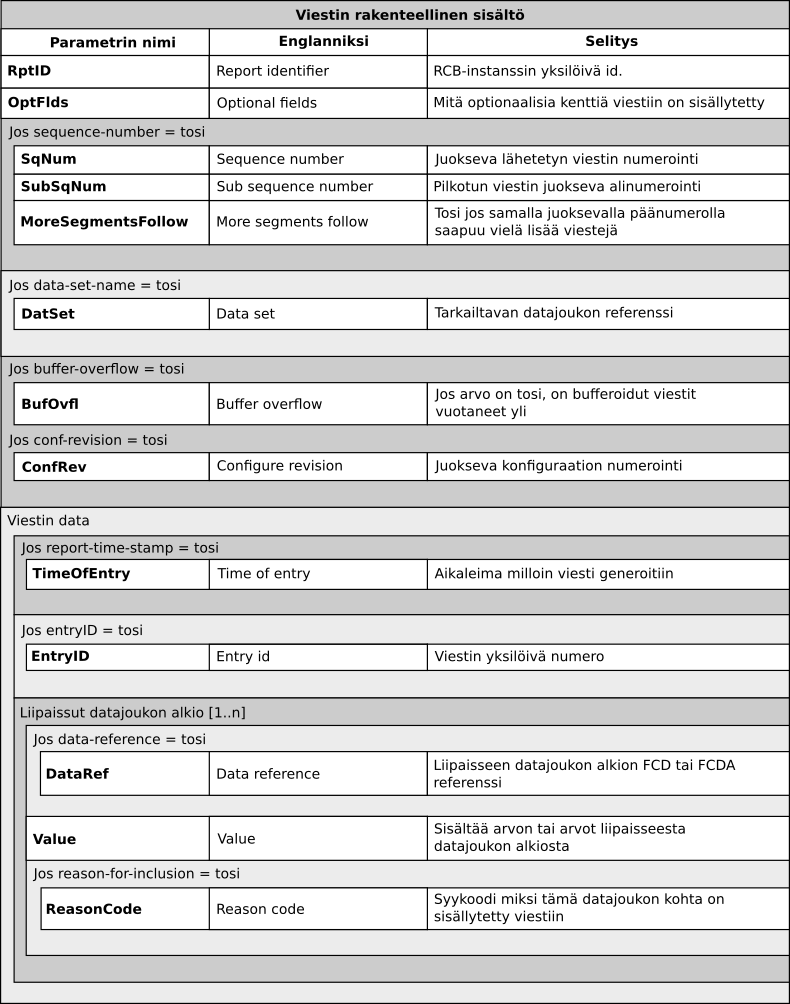
\includegraphics[width=1\textwidth]{pictures/iec61850-report-format.png}
	\caption{Standardin määrittämä lähetetyn viestin rakenne (pohjautuu kuvaan \mbox{\cite[s.~104]{IEC61850-7-2}}).}
	\label{fig:iec61850-report-format}
\end{figure}

Kuvassa \ref{fig:iec61850-data-set-reporting} on esimerkki, jossa kaksi RCB-instanssia lähettävät viestit data-attribuutin muuttuessa. Kuvassa keskellä on kaksi BRCB-instanssia myBRCB01 ja myBRCB02, jotka tarkkailevat datajoukkoja Testi1 ja Testi2 vastaavasti. Data-attribuutissa MyLD""/""XCBR1"".""Pos"".""stVal tapahtuu arvon muutos, joka on sisällytetty kumpaankin datajoukkoon. Liipaistu tapahtuma on data-change, johon RCB-instanssit reagoivat. Kummassakin instanssissa TrgOps sisältää data-change-liipaisimen. Seurauksena on datajoukon viitteen ja kaikki sen viitattujen arvojen lisääminen viestiin. Viitteen kaikki arvot lisätään viestiin, vaikka niistä liipaisee vain yksi. Kuvan alempi viesti sisältää 6 arvoa ja ylempi vain yhden arvon. Syynä on datajoukossa käytetty viite. Testi1-datajoukossa käytetty viite viittaa vain yhteen attribuuttiin ja Testi2-datajoukossa viite viittaa 6 eri attribuuttiin. Kuvasta voi myös nähdä OptFlds-attribuutin vaikutuksen viestin kenttiin. \mbox{\cite[s.~103--109]{IEC61850-7-2}}

\begin{figure}[ht!]
	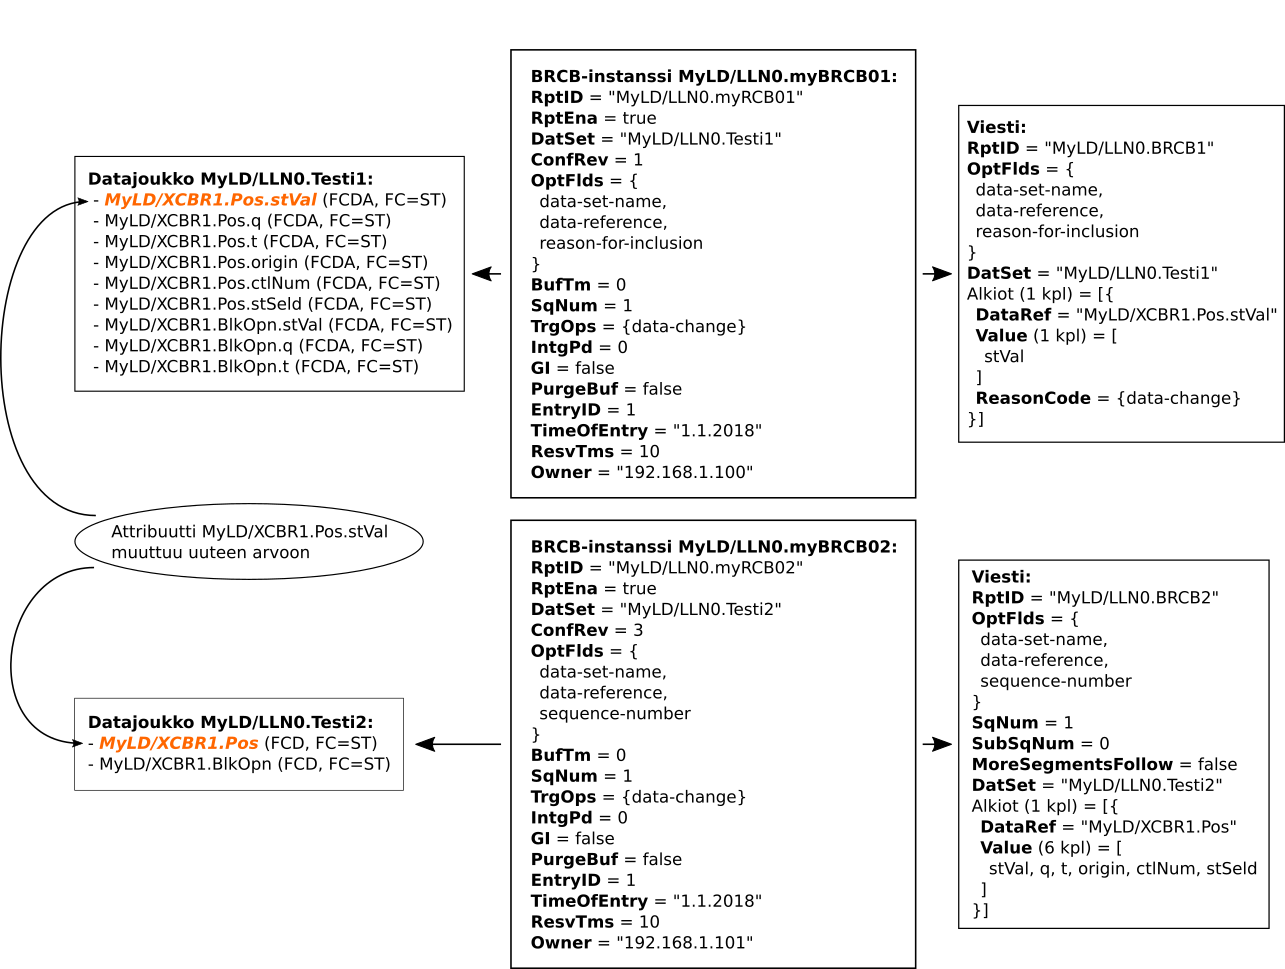
\includegraphics[width=1\textwidth]{pictures/iec61850-data-set-reporting.png}
	\caption{BRCB-instanssi tarkkailee sille määritettyä datajoukkoa ja generoi viestin tapahtuman liipaistessa.}
	\label{fig:iec61850-data-set-reporting}
\end{figure}

% TODO: Typot ja viitteet tästä eteenpäin.

Viestissä \emph{RptID}-kenttä sisältää viitteen RCB-instanssiin, mistä viesti on peräisin. OptFlds sisältää binääritietueen viestin vaihtoehtoisista kentistä. Viestin kenttiä \emph{SqNum}, \emph{SubSqNum} ja \emph{MoreSegmentsFollow} käytetään kertomaan asiakkaalle, jos viesti on liian pitkä. Tällöin viesti ositetaan ja lähetetään monessa osassa, jotka numeroidaan yksilöivästi edelle mainittuilla kentillä. Kenttä \emph{DatSet} sisältää viitteen datajoukkoon mistä viesti on peräisin. Puskuroidussa BRCB-instanssissa kenttä \emph{BufOvlf} kertoo, onko viestipuskuri vuotanut yli. \emph{ConfRev} kertoo juoksevan konfiguraation numeron, tämä tulee suoraan RCB-instanssin samannimisestä attribuutista. \emph{TimeOfEntry} kertoo, milloin viesti generoitiin IED-laitteen päässä. \emph{EntryID} on viestin yksilöivä numerointi. Tämä kenttä tulee suoraan RCB-instanssin samannimisestä kentästä. Tämän jälkeen viestissä tulee taulukko, joka sisältää liipaisseet datajoukon alkiot. Jokainen taulukon alkio sisältää \emph{Value}-kentän ja vaihtoehtoiset \emph{DataRef}- ja \emph{ReasonCode}-kentät. DataRef sisältää datajoukon FCD- tai FCDA-viitteen, joka liipaisi tapahtuman. ReasonCode-kenttä kertoo mikä RCB-instanssin TrgOps-attribuutilla asetetuista liipaisimista liipaisi tapahtuman ja aiheutti alkion sisällytyksen viestiin. Kentän mahdolliset arvot ovat samat kuin RCB-instanssin TrgOps-attribuutin arvot.

Value-kentän arvosta on tärkeä ymmärtää, että se voi sisältää yhden tai monta data-att\-ri\-buu\-tin arvoa. Tämä riippuu siitä, viittaako datajoukon liipaissut alkion FCD- vai FCDA-viitteellä useaan data-attribuuttiin. Viittauksen ollessa FCDA-viite, joka viittaa vain yhteen data-attribuuttiin, sisältää Value-kenttä vain kyseisen data-attribuutin arvon. Jos viittaus on FCD- tai FCDA-viite, joka viittaa moneen attribuuttiin hierarkiassa alaspäin. Sisältää Value-kenttä kaikki nämä arvot, vaikka niistä olisi liipaissut vain yksi attribuutti. FCD- ja FCDA-viittauksen toimintaa ja mitä attribuutteja se viittaa hierarkiassa alaspäin, käydään läpi kappaleessa \ref{ch:fc-and-dataset}. Esimerkki tästä on kuvassa \ref{fig:iec61850-data-set-reporting}, jossa liipaisu yhdessä attribuutissa aiheuttaa eri määrän arvoja kumpaankin viestiin. Tähän vaikuttaa kuinka liipaisevaan attribuuttiin on viitattu datajoukossa. Kuvassa \ref{fig:iec61850-data-set-reporting} Testi1 attribuuttiin MyLD""/""XCBR1"".""Pos"".""stVal on viitattu FCDA-viitteellä, jossa funktionaalinen rajoite on ST. Eli FCDA-viite viittaa vain stVal-attribuuttiin, ei muihin. Tämän takia myBRCB01-instanssilta tuleva viestin Value-kenttä sisältää vain stVal-attribuutin arvon. Datajoukon Testi2 FCD-viite MyLD""/""XCBR1"".""Pos funktionaalisella rajoitteella ST sisältää kaikki Pos-instanssin ST data-attribuutit. Tämä sisältää myös muuttuneen MyLD/XCBR1.Pos.stVal da\-ta""-""att\-ri\-buu\-tin. Tämä aiheuttaa sen, että kaikki datajoukon viitteen MyLD""/""XCBR1"".""Pos viitatut attribuutit lisätään viestiin. BRCB-instanssilta myBRCB02 tuleva viestin Value-kenttä sisältää kaikki viitatut attribuutit ja viestin DatRef-kenttä sisältää datajoukossa käytetyn viitteen. Pos-dataobjektin attribuutit voi tarkistaa taulukosta \ref{tab:iec61850-DPC-class-definition}. \mbox{\cite[s.~40--44]{IEC61850-7-1}} \mbox{\cite[s.~108]{IEC61850-7-2}}


\section{Abstraktimallin sovitus MMS-protokollaan}
\label{ch:iec61850-mms-mallinnus}
Tähän asti käsitellyt IEC 61850 -standardin mallit ja palvelut ovat olleet abstrahoituja ja tekniikasta riippumattomia. Tässä työssä käytetiin IEC 61850 -standardin MMS-protokollan toteutusta. Tästä toteutuksesta on tarkemmin määritetty IEC 61850 -stan\-dar\-din osassa 8-1. MMS-protokolla on maailmanlaajuinen \emph{ISO 9506} -standardi viestintään, joka on määritetty toimivaksi TCP/IP:n pinon päällä \mbox{\cite{MMS-protocol-stack-and-API}}. Tämän työn kannalta lukijan ei tarvitse ymmärtää MMS-protokollaa ja sen toimintaa. Suunnitellussa ohjelmistossa käytettiin apuna kirjastoa, joka hoitaa matalan tason kommunikoinnin IED-laitteen kanssa. Tässä osiossa käsitellään työn kannalta tärkeitä tietoja, mitä toteutuksesta MMS-protokollalle kuitenkin tarvitsee tietää. \mbox{\cite{Introduction-to-the-MMS}}

IEC 61850 -standardin mallinnuksessa aikaisemmin esitetty instanssien viittaus hierarkiassa muuttuu ja nyt viittaus sisältää myös funktionaalisen rajoitteen. Esimerkkinä kuvassa \ref{fig:iec61850-data-reference} oleva viite OmaLD/Q0XCBR1.Pos.stVal funktionaalisella rajoitteella ST muuttuu muotoon OmaLD/Q0XCBR1\$ST\$Pos\$stVal. Tässä viittauksessa pisteet (.) korvataan dollarin merkillä (\$). Ja kaksikirjaiminen funktionaalinen rajoite sijoitetaan loogisen noodin ja ensimmäisen dataobjektin nimien väliin. Muuten viittaus säilyy identtisenä alkuperäiseen, ja samat rajoitteet ja nimeämiskäytännöt ovat voimassa edelleen. \mbox{\cite[s.~34--35, 111]{IEC61850-8-1}}

Tämän uuden viittauksen takia jokaiselle viitattavalle kohteelle täytyy olla funktionaalinen rajoite. Niinpä esimerkiksi RCB-luokkien instansseille täytyy olla myös funktionaalinen rajoite. Puskuroitua RCB-instanssia viitataan funktionaalisella rajoitteella \emph{BR}. Ja puskuroimatonta funktionaalisella rajoitteella \emph{RP}. Esimerkin tästä viittauksesta voi nähdä aikaisemmin mainitusta kuvasta \ref{fig:iec61850-data-set-reporting}. \mbox{\cite[s.~32--34, 75]{IEC61850-8-1}}